%!LW recipe=uplatex

\documentclass[0_main]{subfiles}

\begin{document}

\ifEn
    \section{Quasi-Newton Methods}
\else
    \section{準ニュートン法}
\fi
\label{sec:background_quasi_newton}

\begin{figure}[t]
    \centering
    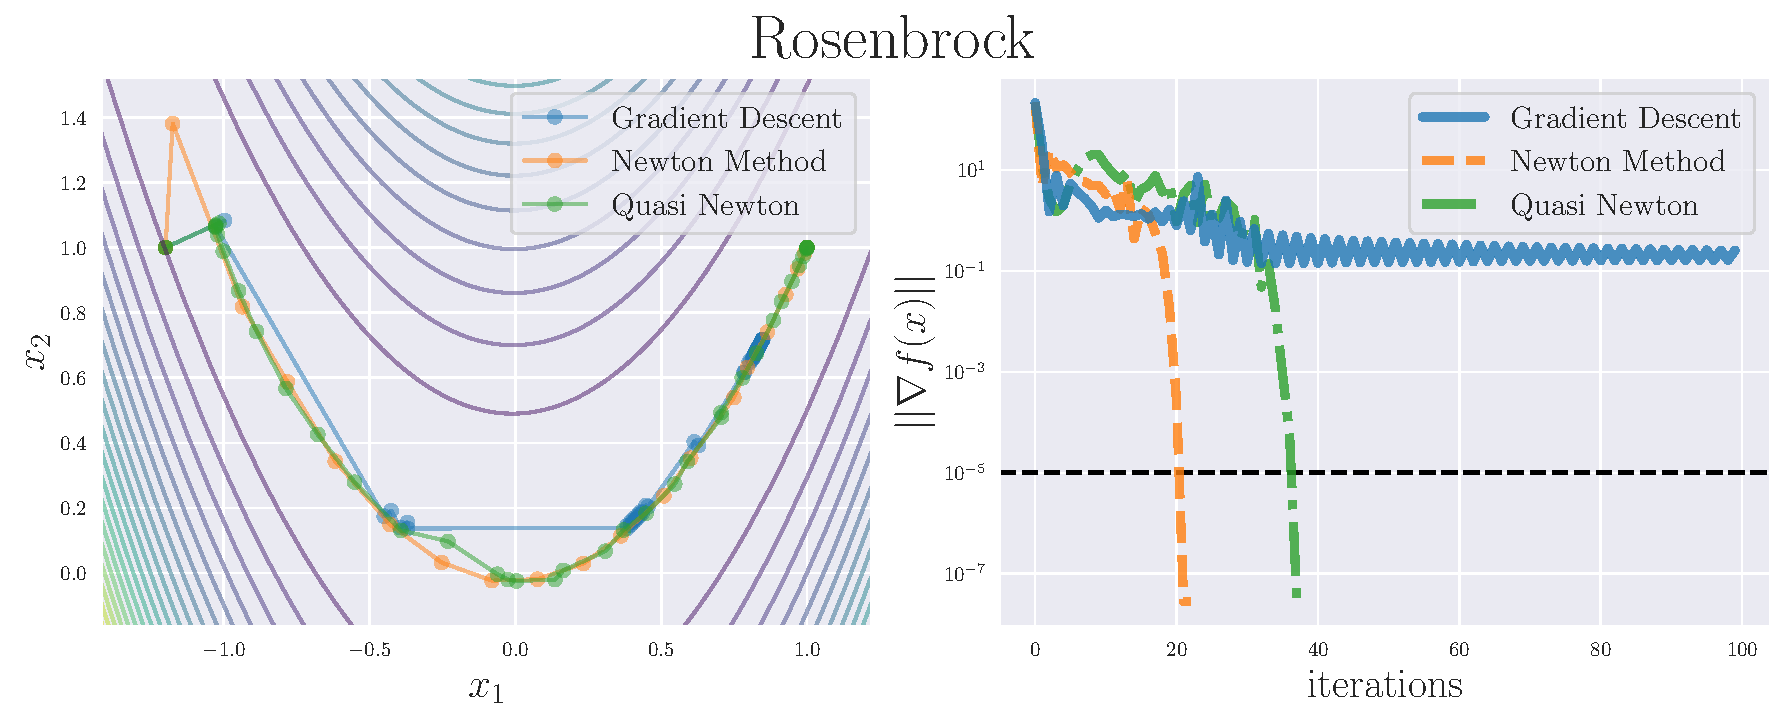
\includegraphics[width=\textwidth]{../imgs/quasi_newton/newton_vs_qs_vs_gd.pdf}
    \caption{
        \ifEn
            Comparison of Newton's method, quasi-Newton methods, and gradient descent
        \else
            ニュートン法、準ニュートン法、勾配降下法の比較
        \fi
    }
    \label{fig:newton_vs_qs_vs_gd}
\end{figure}

\ifEn
    In this section, we discuss quasi-Newton methods. Quasi-Newton methods are based on Newton's method, but aim to reduce its primary drawback, namely, the high computational cost of evaluating the Hessian matrix. Specifically, instead of using the true Hessian matrix $\nabla^2 f(x_k)$, an approximation matrix $B_k$ is employed, thereby achieving fast convergence while keeping the computational cost low.
\else
    本節では準ニュートン法について述べる。準ニュートン法はニュートン法に基づくが、その主要な欠点であるヘッセ行列の計算コストの大きさを低減することを目的とする。具体的には真のヘッセ行列 $\nabla^2 f(x_k)$ の代わりに近似行列 $B_k$ を用い、高速な収束性を保ちつつ計算コストを抑える。
\fi

\ifEn
    \Cref{fig:newton_vs_qs_vs_gd} shows a comparison of Newton's method, quasi-Newton methods, and gradient descent. Gradient descent is a method that simply updates in the direction opposite to the gradient. Although its per-iteration computational cost is the lowest, its convergence is slow. Newton's method converges in the fewest iterations, but has the highest computational cost per step. Quasi-Newton methods lie between these two extremes, striking a balance between them. In particular, when comparing methods in terms of computation time rather than the number of iterations, quasi-Newton methods often exhibit the best performance.
\else
    \Cref{fig:newton_vs_qs_vs_gd} はニュートン法、準ニュートン法、勾配降下法の比較を示す。勾配降下法は勾配の反対方向に単純に更新する方法である。1反復あたりの計算コストは最小だが収束は遅い。ニュートン法は反復回数が最も少ない一方で、1ステップあたりの計算コストが最も高い。準ニュートン法はその中間に位置し、両者のバランスを取る。特に反復回数ではなく計算時間で比較すると、準ニュートン法が最良の性能を示すことが多い。
\fi

\ifEn
    Line-search-based quasi-Newton methods generate a sequence $\{ x_k \}_{k=0}^{\infty}$ converging to the optimal solution $x^*$ as follows:
\else
    線形探索に基づく準ニュートン法は、最適解 $x^*$ に収束する列 $\{ x_k \}_{k=0}^{\infty}$ を次のように生成する:
\fi
\begin{equation*}
    x_{k+1} = x_k - \alpha_k B_k^{-1} \nabla f(x_k)
    = x_k - \alpha_k H_k \nabla f(x_k).
\end{equation*}
\ifEn
    Here, $\alpha_k > 0$ is the step size determined by line search, $B_k$ is an approximation of the Hessian matrix $\nabla^2 f(x_k)$ at the point $x_k$, and $H_k \coloneqq B_k^{-1}$ denotes its inverse.
\else
    ここで $\alpha_k > 0$ は線形探索で定めるステップサイズであり、$B_k$ は点 $x_k$ におけるヘッセ行列 $\nabla^2 f(x_k)$ の近似である。$H_k \coloneqq B_k^{-1}$ はその逆行列を表す。
\fi

\begin{figure}[t]
    \begin{minipage}{0.33\textwidth}
        \centering
        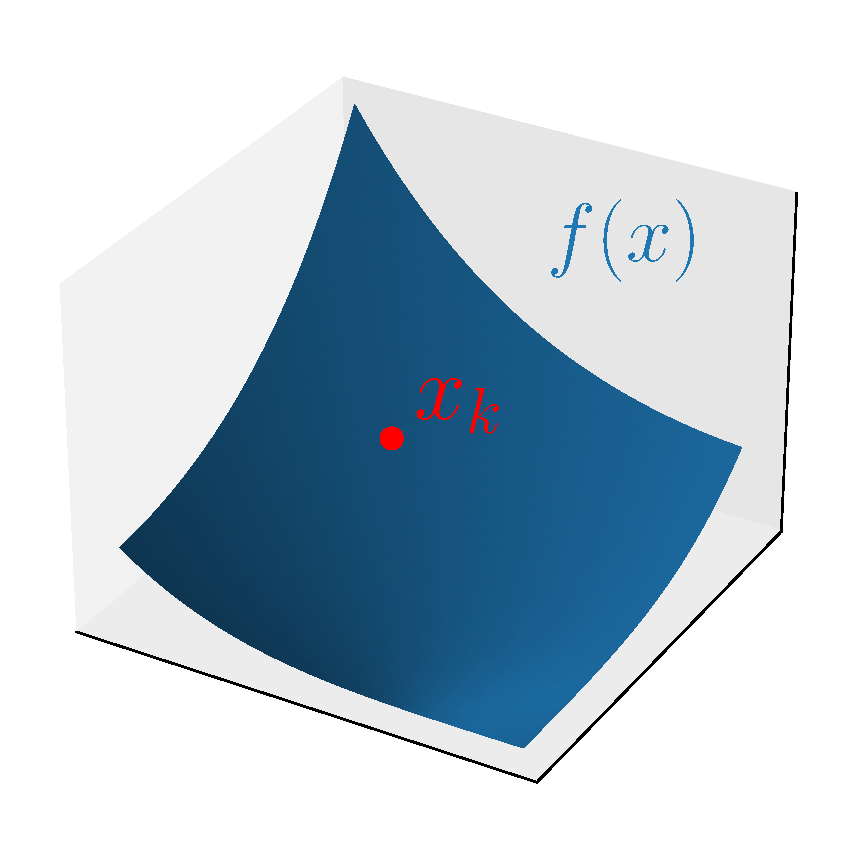
\includegraphics[width=\textwidth]{../imgs/quasi_newton/quasi_newton_1.pdf}
    \end{minipage}%
    \begin{minipage}{0.33\textwidth}
        \centering
        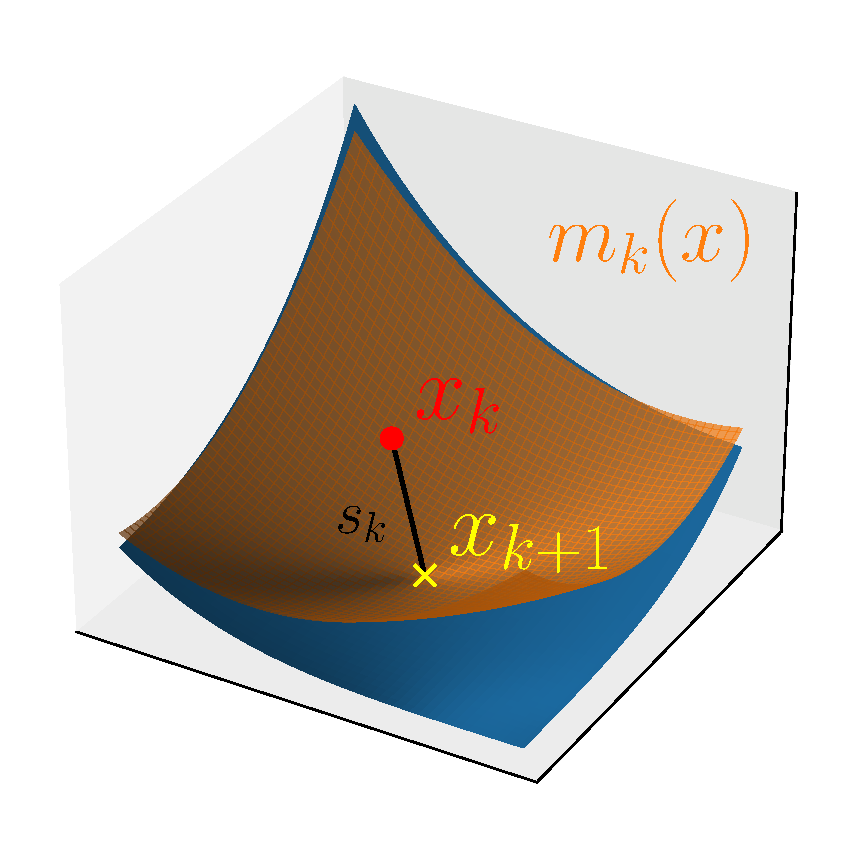
\includegraphics[width=\textwidth]{../imgs/quasi_newton/quasi_newton_2.pdf}
    \end{minipage}%
    \begin{minipage}{0.33\textwidth}
        \centering
        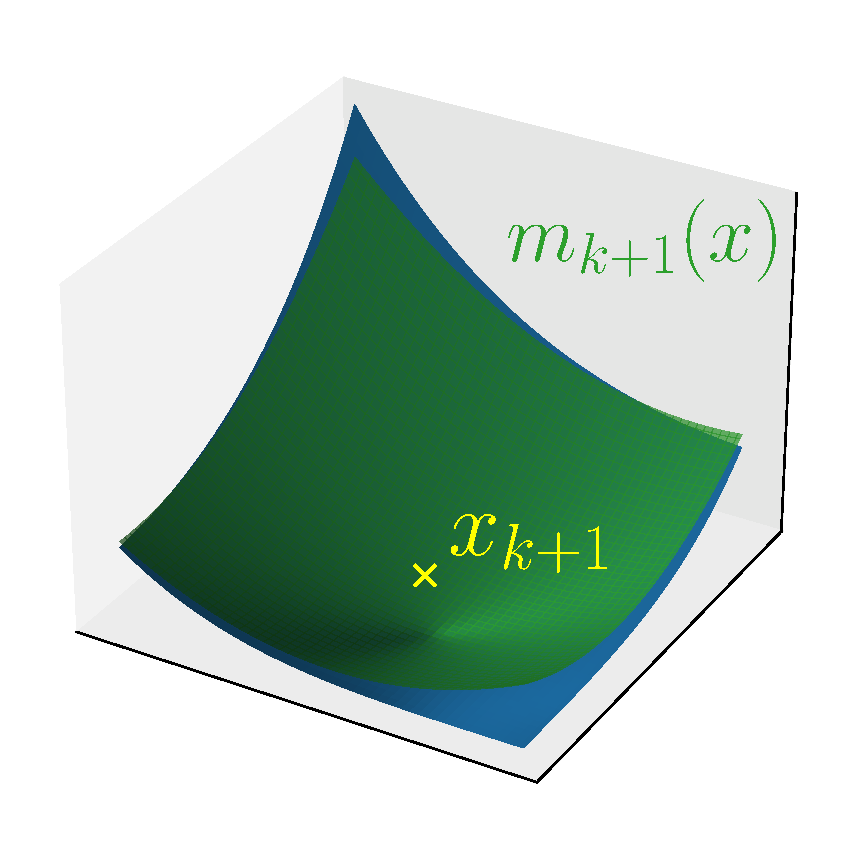
\includegraphics[width=\textwidth]{../imgs/quasi_newton/quasi_newton_3.pdf}
    \end{minipage}
    \caption{
        \ifEn
            Conceptual illustration of quasi-Newton methods.
            (1) Given the objective function $f$ (blue surface) and the current point $x_k$ (red point).
            (2) Move to the minimizer $x_{k+1}$ (yellow cross) of the quadratic model $m_k(x)$ (orange surface) obtained by the current approximate Hessian.
            (3) Update the quadratic model (green surface) and repeat this operation.
        \else
            準ニュートン法の概念図。
            (1) 目的関数 $f$ (青い曲面) と現在点 $x_k$ (赤点)が与えられる。
            (2) 現在の近似ヘッセ行列によって得られる二次モデル $m_k(x)$ (橙色の曲面) にて、その最小点 $x_{k+1}$ (黄色のバツ印) に移動する。
            (3) 二次モデルを更新し (緑色の曲面)、この操作を繰り返す。
        \fi
    }
    \label{fig:quasi_newton_overview}
\end{figure}

\ifEn
    The core of quasi-Newton methods lies in how to update $B_k$ at each iteration so that it approaches the true Hessian matrix.
    \Cref{fig:quasi_newton_overview} illustrates this concept. First, around the current point $x_k$, a quadratic approximation model of the objective function $f$ is constructed using $B_k$. Next, this quadratic model is minimized to obtain the next point $x_{k+1}$. After obtaining $x_{k+1}$, the approximation matrix $B_k$ is updated to $B_{k+1}$ using the gradient information at $x_k$ and $x_{k+1}$. This procedure is repeated until convergence, which constitutes the quasi-Newton method.
\else
    準ニュートン法の核心は、各反復で $B_k$ をどのように更新して真のヘッセ行列に近づけるかにある。\Cref{fig:quasi_newton_overview} はこの概念を示す。まず現在点 $x_k$ の周りで、$B_k$ を用いて目的関数 $f$ の二次近似モデルを構成する。次にこの二次モデルを最小化して次の点 $x_{k+1}$ を得る。$x_{k+1}$ を得た後、$x_k$ と $x_{k+1}$ における勾配情報を用いて近似行列 $B_k$ を $B_{k+1}$ に更新する。この手続きを収束まで繰り返すことが準ニュートン法である。
\fi

\ifEn
    \subsection{Secant Condition}
\else
    \subsection{セカント条件}
\fi

\ifEn
    Let $f\colon \mathbb{R}^n \to \mathbb{R}$ be of class $C^2$.
    Suppose that a symmetric matrix $B_k$ is given as an approximation of the Hessian matrix $\nabla^2 f(x_k)$.
    We determine an approximate Hessian $B_{k+1}$ at the next point $x_{k+1}$.
    Although there are infinitely many possible candidates for such a matrix, it is natural to impose symmetry on $B_{k+1}$, given that the true Hessian matrix is symmetric.
    For the current point $x_k$ and the next point $x_{k+1}$,
    we define the step and gradient difference as
\else
    関数 $f\colon \mathbb{R}^n \to \mathbb{R}$ を $C^2$ 級とする。
    対称行列 $B_k$ が点 $x_k$ におけるヘッセ行列 $\nabla^2 f(x_k)$ の近似として与えられているとする。
    次の点 $x_{k+1}$ における近似ヘッセ行列 $B_{k+1}$ を定める。
    このような行列の候補は無数に存在するが、真のヘッセ行列が対称であることから $B_{k+1}$ にも対称性を課すのが自然である。
    現在点 $x_k$ と次点 $x_{k+1}$ に対して、ステップと勾配差を次で定義する。
\fi
\begin{equation*}
    s_k \coloneq x_{k+1} - x_k, \qquad   y_k \coloneq \nabla f(x_{k+1}) - \nabla f(x_k).
\end{equation*}
\ifEn
    We assume that $y_k^\top s_k \neq 0$ and $s_k \neq 0$.
    Here, the $s$ in $s_k$ stands for step.
    Since the new approximation is constructed around $x_{k+1}$, we consider approximating $\nabla f(x_k)$ using the Hessian matrix $\nabla^2 f(x_{k+1})$ and $B_{k+1}$ as follows:
\else
    $y_k^\top s_k \neq 0$ かつ $s_k \neq 0$ を仮定する。なお、$s_k$ の $s$ は step を意味する。
    ここで、新しい近似は $x_{k+1}$ を中心に構築されるため、$\nabla f(x_k)$ をヘッセ行列 $\nabla^2 f(x_{k+1})$ および $B_{k+1}$ を用いて近似することを考える。
\fi
\begin{align*}
    \nabla f(x_k) & \approx \nabla f(x_{k+1}) + \nabla^2 f(x_{k+1})(x_k - x_{k+1}) \\
                  & \approx \nabla f(x_{k+1}) + B_{k+1}(x_k - x_{k+1})
\end{align*}
\ifEn
    Requiring the above approximation to hold as an equality yields
\else
    上の近似を等式として要求すると次を得る。
\fi
\begin{equation*}
    B_{k+1}(x_{k+1} - x_k) = \nabla f(x_{k+1}) - \nabla f(x_k),
\end{equation*}
\ifEn
    or equivalently,
\else
    あるいは同値に
\fi
\begin{equation*}
    B_{k+1} s_k = y_k.
\end{equation*}
\ifEn
    This relation is called the secant condition, or the quasi-Newton equation.
\else
    この関係はセカント条件、または準ニュートン方程式と呼ばれる。
\fi

\ifEn
    More precisely, the secant condition can also be justified as follows. Consider a quadratic approximation model around $x_{k+1}$:
\else
    より厳密には、セカント条件は次のように正当化することも出来る。$x_{k+1}$ の周りの二次近似モデルを考える。
\fi
\begin{equation*}
    m_{k+1}(x) = f(x_{k+1}) + \nabla f(x_{k+1})^\top (x - x_{k+1}) + \frac{1}{2} (x - x_{k+1})^\top B_{k+1} (x - x_{k+1}).
\end{equation*}
\ifEn
    By construction, regardless of $B_{k+1}$, this model satisfies
\else
    このモデルは構成上、$B_{k+1}$と関係なしに、次を満たす:
\fi
\begin{equation*}
    \begin{cases}
        m_{k+1}(x_{k+1}) = f(x_{k+1}), \\
        \nabla m_{k+1}(x_{k+1}) = \nabla f(x_{k+1}).
    \end{cases}
\end{equation*}
\ifEn
    Additionally, the secant condition ensures that the model satisfies
\else
    さらに、セカント条件はモデルが次を満たすことを保証する:
\fi
\begin{align*}
    \nabla m_{k+1}(x_k) & = \nabla f(x_{k+1}) - B_{k+1} (x_{k+1} - x_k)             &  & (\text{definition of model}) \\
                        & = \nabla f(x_{k+1}) - (\nabla f(x_{k+1}) - \nabla f(x_k)) &  & \text{(secant condition)}    \\
                        & = \nabla f(x_k).
\end{align*}
\ifEn
    This implies that the secant condition ensures that the quadratic model $m_{k+1}(x)$ accurately reflects the known information at both $x_{k+1}$ and $x_k$, except for the previous function value $f(x_k)$.
\else
    これはセカント条件が、二次モデル $m_{k+1}(x)$ が既知の情報を $x_{k+1}$ と $x_k$ の両方を、前の関数値 $f(x_k)$ を除いて、正確に反映していることを意味する。
\fi

\end{document}
